\documentclass[12pt]{article}
\usepackage{datetime}
\usepackage{acronym}
\usepackage{xcolor}
\setlength {\marginparwidth }{2cm}
\usepackage{todonotes}
\usepackage{hyperref}
\usepackage{amsmath}
\usepackage{subcaption}
\usepackage{tikz}
\usetikzlibrary{arrows,shapes.geometric,positioning,automata,calc}
% \usepackage{textcomp}
% \usepackage{mathrsfs}  % mathscr font
% \usepackage[colorlinks, filecolor=dark_blue, urlcolor=dark_blue, linkcolor=black, citecolor=black]{hyperref}

\usepackage[backend=biber]{biblatex}
\addbibresource{bibliography.bib}
\usepackage{cleveref}

\newcommand{\meta}[1]{{\color{blue}#1}}  

\newdateformat{monthyeardate}{\monthname[\THEMONTH], \THEYEAR}

\acrodef{iot}[IoT]{Internet of Things}
\acrodef{cps}[CPS]{Cyber-Physical System}
\acrodef{ac}[AC]{Aggregate Computing}
\acrodef{qos}[QoS]{Quality of Service}
\acrodef{cas}[CAS]{Collective Adaptive Systems}
\acrodef{api}[API]{Application Programming Interface}
\acrodef{iac}[IaC]{Infrastructure as Code}
\acrodef{ci}[CI]{Continuous Integration}
\acrodef{ai}[AI]{Artificial Intelligence}
\acrodef{dl}[DL]{Deep Learning}

\begin{document}

\begin{titlepage}
	\centering

	\textsc{\Large Ph.D Programme in Computer Science and Engineering}\\[0.5cm]
	\textsc{\Large Admission XXXIX Cycle}\\[0.6cm]

	\hrule width \hsize \kern 1mm \hrule width \hsize height 2pt
	\vspace{0.8cm}

	{\large \bfseries Research Project Proposal}\\[0.6cm]
	{\large \emph{Engineering Reconfigurable Collective Systems in Cloud-Edge Environments}}\\[0.6cm]

	{\bfseries{\monthyeardate\today} \hfill \bfseries{Nicolas Farabegoli}}\\[0.6cm]

	\hrule width \hsize height 2pt \kern 1mm \hrule width \hsize height 1pt
	\vspace{0.4cm}

	\begin{abstract}
		% Da riscrivere in alcuni punti
		In recent years,
		the emergence of \ac{cps} has engendered a noteworthy surge in complexity and heterogeneity
		within the underlying infrastructure supporting these systems.
		Notably, the interplay between cloud, fog, and edge computing exemplifies the intricacy inherent in such systems.
		%
		Modern collective adaptive applications like \ac{iot}, human enhanced by wearable devices,
		swarm robotics, smart cities,
		are designed to be executed on several devices and to be deployed in
		heterogeneous infrastructures, ranging from cloud servers to wearable devices.
		%
		The availability of such a wide range of devices and infrastructures opens to
		better exploitation of the available resources and performance,
		but introduces complexity in the design and deployment of such applications.
		%
		This research project proposes to produce a framework for the design and deployment of
		collective adaptive applications on heterogeneous infrastructures.
		%
		Reconfiguration aspects will be considered,
		allowing the application to adapt to the changes in the infrastructure and external conditions.
		%
		The framework will leverage machine learning techniques to manage the complex task of reconfiguration
		to opportunistically balance the performance and energy consumption.
		%
		The framework will also offer modern approaches to make data available enabling data analysis;
		it becomes necessary because of the large amount of data produced by the \ac{iot} devices from extremely scattered data sources.
		%
		% With numerous \ac{iot} devices and vast amounts of data from various sources,
		% the framework ensures consistent data access for comprehensive analysis.
		% Since the \ac{iot} consists of a large number of devices,
		% they produce a large amount of data from extremely scattered data sources.
		% %
		% The management of such data is a complex and delicate task,
		% which will be addressed with state-of-the-art techniques.
	\end{abstract}
\end{titlepage}

\section{State of the Art}\label{sec:state-of-the-art}

\paragraph{Collective Adaptive Systems}
A \ac{cas} is a system composed of several entities that interact with each other and can dynamically adapt to changing environments or requirements~\cite{DBLP:conf/birthday/HolzlW11}.
%
Often,
the entities of these systems have their own goals and objectives,
and interactions with other entities or may lead to unexpected phenomena.
%
Many modern systems are collective adaptive systems: \emph{smart cities}, \emph{collective cyber-physical systems}, \emph{robot swarms} and \emph{sensor network}.
%
The notion of \ac{cas} was elaborated in the workshop ``Fundamentals of Collective Adaptive Systems''~\cite{DBLP:journals/corr/abs-1108-5643}
organized by the European Commission in 2009,
and in the following years,
it has been the subject of several research projects~\cite{DBLP:journals/procedia/ZambonelliCFMRSRTDSYNOMVFMW11,DBLP:series/lncs/8998}.

Coordination in \ac{cas} is a fundamental aspect to consider when adaptation properties are required.
%
Coordination~\cite{DBLP:journals/csur/Ciancarini96} represents an effective way to achieve a global goal in a distributed system.
%
When entities of the system start to communicate with each other,
the need for coordination arises.
%
In the literature,
there are several approaches to coordination~\cite{DBLP:journals/csur/Ciancarini96}:
\emph{message passing}, \emph{tuple space models}~\cite{DBLP:books/sp/omicini01/RossiCD01}, \emph{stigmergy models}~\cite{DBLP:journals/cogsr/Heylighen16}.

In several pervasive systems,
the traditional approaches in the engineering of these systems are not suitable,
due to the lack of mechanisms to address complex behaviour and limited scalability.

Situatedness and time awareness are two important aspects of pervasive systems.
%
For this reason,
spatial computing has emerged to manage these aspects as a first-class citizen~\cite{Beal_Viroli_2015}.
%
This approach makes it possible to obtain self-adaptive properties in the system,
and react to changes in the environment and faults conditions.

\ac{ac}~\cite{DBLP:journals/computer/BealPV15} is a novel approach that consists in manipulating computational fields,
in a declarative and compositional way.
%
This approach shifts the focus from a local perspective to a global one,
where a group of devices can be seen as a single entity in which the aggregate program is executed.
%
The main abstraction on which \ac{ac} is based is the \emph{computational field} i.e.,
a distributed data structure in which each device is mapped to a computational value.

One of the main benefits of this approach is the possibility to focus on high-level aspects and characteristics of the system,
without worrying about low-level details like communication, failure, distribution, and so on.
%
All the low-level aspects are managed by the underlying platform which manages the deployment and execution of the aggregate program.

\paragraph{Pulverisation}
To tackle the complexity of the deployment of \ac{cas},
several approaches have been proposed in the literature.
%
Some examples are: \emph{Osmotic Computing}~\cite{DBLP:journals/tiot/NehaPSSG22}, \emph{multi-tier programming}~\cite{DBLP:journals/csur/WeisenburgerWS20}.

\emph{Pulverisation}~\cite{DBLP:journals/fi/CasadeiPPVW20} represents an approach to distributed application partitioning and deployment.
%
Its goal is to provide a way to specify the functional semantics of the software in a deployment-independent way.
%
To do so,
the application logic should be designed considering a logical system,
which is a set of logical devices forming an arbitrary network topology.
%
The application of each logical device is decomposed into an ensemble of components,
representing respectively a set of \emph{sensors},
a set of \emph{actuators},
a \emph{state},
a \emph{communication} component and a \emph{computation} component modeling the behaviour of the device (see~\Cref{fig:pulv}).
%
\begin{figure}
	\tikzset{-,
		host/.style={rectangle,draw,line width={2pt},inner sep=10pt,
				outer sep=0, minimum height=1.5cm, minimum width=1.8cm, %text height=0.2cm, 
				text depth=0.5cm,
				fill=black!10!white
			},
		node/.style={rectangle,draw,dotted,line width={1pt}, inner sep=2pt,
				fill=blue!20!white,
				font=\large
			},
		nodeA/.style={node,fill=red!20!white},
		nodeB/.style={node,fill=green!20!white},
		nodeC/.style={node,fill=black!30!white},
		nodeD/.style={node,fill=white!20!white},
		plink/.style={line width=2pt},
		llink/.style={dotted,line width=2pt,red},
		hostThin/.style={rectangle,draw,line width={0.5pt},inner sep=10pt,
				outer sep=0, minimum height=1.1cm, minimum width=1.8cm, %text height=0.2cm, 
				text depth=0.5cm,
				fill=black!10!white
			},
		lnode/.style={node,minimum width=0.55cm,minimum height=0.55cm},
		loglink/.style={->,line width=1.5pt}
	}
	\def\nm{0.35cm} %nm = node margin offset
	\def\tpscale{0.7}
	\newcommand{\agent}{device}
	\newcommand{\LSens}{\boldsymbol{\sigma}}
	\newcommand{\LComp}{\boldsymbol{\beta}}
	\newcommand{\LComm}{\boldsymbol{\chi}}
	\newcommand{\LAct}{\boldsymbol{\alpha}}
	\newcommand{\LState}{\boldsymbol{\kappa}}

	\begin{minipage}{\columnwidth}
		\centering
		\begin{tikzpicture}[every node/.style={scale=0.85}]
			\node[hostThin,minimum width=3.4cm,minimum height=3cm,dashed]
			(h1) [label={[yshift=0.35cm]above:{\textbf{logical \agent{}}}}] {};

			\node[lnode] (d1) at (h1.north west) [xshift=\nm,yshift=-\nm,label=above:{behaviour}] {$\LComp$};
			\node[lnode] (d2) at (h1.north east) [xshift=-\nm,yshift=-\nm,label=above:{communication}] {$\LComm$};
			\node[lnode] (d3) at (h1.center) [xshift=0,yshift=0,label=right:{state/knowledge}] {$\LState$};
			\node[lnode] (d4) at (h1.south west) [xshift=\nm,yshift=\nm,label=below:{sensors}] {$\LSens$};
			\node[lnode] (d5) at (h1.south east) [xshift=-\nm,yshift=\nm,label=below:{actuators}] {$\LAct$};

			\node[hostThin,minimum width=2.3cm,minimum height=2.3cm,dashed]
			(h2) [right=2cm of h1, label={above:{\textbf{neighbour \agent{}}}}] {};

			\node[lnode] (d21) at (h2.north west) [xshift=\nm,yshift=-\nm] {$\LComm$};
			\node[lnode] (d22) at (h2.north east) [xshift=-\nm,yshift=-\nm] {$\LComp$};
			\node[lnode] (d23) at (h2.center) [xshift=0,yshift=0] {$\LState$};
			\node[lnode] (d24) at (h2.south west) [xshift=\nm,yshift=\nm] {$\LSens$};
			\node[lnode] (d25) at (h2.south east) [xshift=-\nm,yshift=\nm] {$\LAct$};

			\draw[loglink] (d1) -- (d3);
			\draw[loglink] (d2) -- (d3);
			\draw[loglink] (d3) -- (d1);
			\draw[loglink] (d3) -- (d2);
			\draw[loglink] (d4) -- (d3);
			\draw[loglink] (d3) -- (d5);

			\draw[loglink] (d21) -- (d23);
			\draw[loglink] (d22) -- (d23);
			\draw[loglink] (d23) -- (d21);
			\draw[loglink] (d23) -- (d22);
			\draw[loglink] (d24) -- (d23);
			\draw[loglink] (d23) -- (d25);

			\draw[loglink] (d2.east) -- (d21.west);
			\draw[loglink] (d21.west) -- (d2.east);


		\end{tikzpicture}
		\subcaption{A logical device, split into sub-components, and one of its neighbours.\label{fig:pulv:dev}}
	\end{minipage}
	\\[0.2cm]
	\begin{minipage}{\columnwidth}
		\def\nm{0.3cm} %nm = node margin offset

		\begin{minipage}{0.48\columnwidth}\centering
			\begin{tikzpicture}[node distance=1.0cm and 0.5cm,every node/.style={scale=\tpscale}]
				% physical nodes
				\node[host] (h1) [anchor=north,label=above:{}] {};
				\node[host] (h2) [right=of h1,label=above:{}] {};
				\node[host] (h3) [below=of h1, label=above:{}] {};
				\node[host] (h4) [right=of h3, label=above:{}] {};

				\node[node] (n11) at (h1.south west) [xshift=\nm,yshift=\nm] {$\LSens$};
				\node[node] (n12) at (h1.south east) [xshift=-\nm,yshift=\nm] {$\LComm$};
				\node[node] (n13) at (h1.north east) [xshift=-\nm,yshift=-\nm] {$\LAct$};
				\node[node] (n14) at (h1.north west) [xshift=\nm,yshift=-\nm] {$\LComp$};
				\node[node] (n15) at (h1) [] {$\LState$};
				% logical node 2
				\node[nodeA] (n21) at (h2.south west) [xshift=\nm,yshift=\nm] {$\LComm$};
				\node[nodeA] (n22) at (h2.south east) [xshift=-\nm,yshift=\nm] {$\LAct$};
				\node[nodeA] (n23) at (h2.north east) [xshift=-\nm,yshift=-\nm] {$\LSens$};
				\node[nodeA] (n24) at (h2.north west) [xshift=\nm,yshift=-\nm] {$\LComp$};
				\node[nodeA] (n25) at (h2) [] {$\LState$};
				% logical node 3
				\node[nodeB] (n31) at (h3.south west) [xshift=\nm,yshift=\nm] {$\LSens$};
				\node[nodeB] (n32) at (h3.south east) [xshift=-\nm,yshift=\nm] {$\LAct$};
				\node[nodeB] (n33) at (h3.north east) [xshift=-\nm,yshift=-\nm] {$\LComm$};
				\node[nodeB] (n34) at (h3.north west) [xshift=\nm,yshift=-\nm] {$\LComp$};
				\node[nodeB] (n35) at (h3) [] {$\LState$};
				% logical node 4
				\node[nodeC] (n41) at (h4.south west) [xshift=\nm,yshift=\nm] {$\LSens$};
				\node[nodeC] (n42) at (h4.south east) [xshift=-\nm,yshift=\nm] {$\LAct$};
				\node[nodeC] (n43) at (h4.north east) [xshift=-\nm,yshift=-\nm] {$\LComp$};
				\node[nodeC] (n44) at (h4.north west) [xshift=\nm,yshift=-\nm] {$\LComm$};
				\node[nodeC] (n45) at (h4) [] {$\LState$};

				% physical links
				\draw[plink]
				(h1) -- (h2)
				(h2) -- (h3)
				(h2) -- (h4)
				(h3) -- (h4)
				;
				% logical links
				\draw[llink]
				(n12) to [] (n21)
				(n21) to [] (n44)
				(n21) to [bend right=30] (n33)
				(n33) to [] (n44);
			\end{tikzpicture}
			\subcaption{Peer-to-peer architecture: one-to-one mapping between logical and physical devices, with no offloading.\label{fig:pulv:p2p}}
		\end{minipage}
		%\hfill
		%\begin{minipage}{0.48\columnwidth}\centering
		%\begin{tikzpicture}[node distance=1.0cm and 0.5cm,
		%every node/.style={scale=\tpscale}]
		%
		%% physical nodes
		%\node[host,minimum width=1.5cm] (h1) [anchor=north,label=above:{}] {};
		%\node[host,minimum width=1.5cm] (h2) [right=of h1,label=above:{}] {};
		%\node[host,minimum width=1.5cm] (h3) [right=of h2, label=above:{}] {};
		%\node[host,minimum width=2.5cm] (he) [above right=0.6cm and -1cm of h1,label=above:{}] {};
		%\node[host,minimum width=3.5cm] (h5) [above=2.6cm of h2,label=right:{}] {};
		%
		%\node[node] (n11) at (h1.south west) [xshift=\nm,yshift=\nm] {$\LSens$};
		%\node[node] (n12) at (h1.south east) [xshift=-\nm,yshift=\nm] {$\LAct$};
		%\node[node] (n13) at (h1.north east) [xshift=-\nm,yshift=-\nm] {$\LState$};
		%\node[node] (n14) at (h1.north west) [xshift=\nm,yshift=-\nm] {$\LComp$};
		%\node[node] (n15) at (he) [xshift=-2*\nm] {$\LComm$};
		%% logical node 2
		%\node[nodeA] (n21) at (h2.south west) [xshift=\nm,yshift=\nm] {$\LSens$};
		%\node[nodeA] (n22) at (h2.south east) [xshift=-\nm,yshift=\nm] {$\LAct$};
		%\node[nodeA] (n23) at (h2.north east) [xshift=-\nm,yshift=-\nm] {$\LState$};
		%\node[nodeA] (n24) at (h2.north west) [xshift=\nm,yshift=-\nm] {$\LComp$};
		%\node[nodeA] (n25) at (he) [xshift=0] {$\LComm$};
		%% logical node 3
		%\node[nodeB] (n31) at (h3.south west) [xshift=\nm,yshift=\nm] {$\LSens$};
		%\node[nodeB] (n32) at (h3.south east) [xshift=-\nm,yshift=\nm] {$\LAct$};
		%\node[nodeB] (n33) at (h3.north east) [xshift=-\nm,yshift=-\nm] {$\LState$};
		%\node[nodeB] (n34) at (h3.north west) [xshift=\nm,yshift=-\nm] {$\LComp$};
		%\node[nodeB] (n35) at (h5) [xshift=2*\nm] {$\LComm$};
		%
		%% physical links
		%\draw[plink] 
		%	(h1) -- (he)
		%	(h2) -- (he)
		%	(h3) -- (h5)
		%	(he) -- (h5);
		%
		%\draw[llink]
		%    %(n15) to [bend left=20] (n35)
		%    (n25) to [bend left=30] (n35);
		%\end{tikzpicture}
		%\subcaption{Communication component offloaded.\label{fig:pulv:comm}}
		%\end{minipage}
		%\\[0.2cm]
		%\begin{minipage}{0.48\columnwidth}\centering
		%\begin{tikzpicture}[node distance=1.0cm and 0.5cm,
		%every node/.style={scale=\tpscale}]
		%
		%% physical nodes
		%\node[host,minimum width=1.5cm] (h1) [anchor=north,label=above:{}] {};
		%\node[host,minimum width=1.5cm] (h2) [right=of h1,label=above:{}] {};
		%\node[host,minimum width=1.5cm] (h3) [right=of h2, label=above:{}] {};
		%\node[host,minimum width=2.5cm] (he) [above right=0.6cm and -1cm of h1,label=above:{}] {};
		%\node[host,minimum width=3.5cm] (h5) [above=2.6cm of h2,label=right:{}] {};
		%
		%\node[node] (n11) at (h1.south west) [xshift=\nm,yshift=\nm] {$\LSens$};
		%\node[node] (n12) at (h1.south east) [xshift=-\nm,yshift=\nm] {$\LAct$};
		%\node[node] (n13) at (he.north) [xshift=-2*\nm,yshift=-\nm] {$\LComm$};
		%\node[node] (n14) at (h1.north) [yshift=-\nm] {$\LComp$};
		%\node[node] (n15) at (he.south) [xshift=-2*\nm,yshift=\nm] {$\LState$};
		%% logical node 2
		%\node[nodeA] (n21) at (h2.south west) [xshift=\nm,yshift=\nm] {$\LSens$};
		%\node[nodeA] (n22) at (h2.south east) [xshift=-\nm,yshift=\nm] {$\LAct$};
		%\node[nodeA] (n23) at (he.north) [xshift=0*\nm,yshift=-\nm] {$\LComm$};
		%\node[nodeA] (n24) at (h2.north) [yshift=-\nm] {$\LComp$};
		%\node[nodeA] (n25) at (he.south) [xshift=0,yshift=\nm] {$\LState$};
		%% logical node 3
		%\node[nodeB] (n31) at (h3.south west) [xshift=\nm,yshift=\nm] {$\LSens$};
		%\node[nodeB] (n32) at (h3.south east) [xshift=-\nm,yshift=\nm] {$\LAct$};
		%\node[nodeB] (n33) at (h5.south) [xshift=2*\nm,yshift=\nm] {$\LComm$};
		%\node[nodeB] (n34) at (h3.north) [yshift=-\nm] {$\LComp$};
		%\node[nodeB] (n35) at (h5.south) [xshift=4*\nm,yshift=\nm] {$\LState$};
		%
		%% physical links
		%\draw[plink] 
		%	(h1) -- (he)
		%	(h2) -- (he)
		%	(h3) -- (h5)
		%	(he) -- (h5);
		%
		%\draw[llink]
		%    %(n15) to [bend left=20] (n35)
		%    (n23) to [bend left=20] (n33);
		%\end{tikzpicture}
		%\subcaption{Communication and state components offloaded.\label{fig:pulv:state}}
		%\end{minipage}
		\hfill
		\begin{minipage}{0.48\columnwidth}\centering
			\begin{tikzpicture}[node distance=1.0cm and 0.5cm,
					every node/.style={scale=\tpscale}]

				% physical nodes
				\node[hostThin,minimum width=1.5cm] (h1) [anchor=north,label=above:{}] {};
				\node[hostThin,minimum width=1.5cm] (h2) [right=of h1,label=above:{}] {};
				\node[hostThin,minimum width=1.5cm] (h3) [right=of h2, label=above:{}] {};
				\node[host,minimum width=2.5cm] (he) [above right=0.6cm and -1cm of h1,label=above:{}] {};
				\node[host,minimum width=3.5cm] (h5) [above=2.6cm of h2,label=right:{}] {};

				\node[node] (n11) at (h1.south west) [xshift=\nm,yshift=\nm] {$\LSens$};
				\node[node] (n12) at (h1.south east) [xshift=-\nm,yshift=\nm] {$\LAct$};
				\node[node] (n13) at (he.south east) [xshift=-4*\nm,yshift=\nm] {$\LComm$};
				\node[node] (n14) at (he.south west) [xshift=1*\nm,yshift=\nm] {$\LComp$};
				\node[node] (n15) at (he.north) [xshift=-2*\nm,yshift=-\nm] {$\LState$};
				% logical node 2
				\node[nodeA] (n21) at (h2.south west) [xshift=\nm,yshift=\nm] {$\LSens$};
				\node[nodeA] (n22) at (h2.south east) [xshift=-\nm,yshift=\nm] {$\LAct$};
				\node[nodeA] (n23) at (he.south east) [xshift=-2.5*\nm,yshift=\nm] {$\LComm$};
				\node[nodeA] (n24) at (he.south west) [xshift=2.5*\nm,yshift=\nm] {$\LComp$};
				\node[nodeA] (n25) at (he.north) [xshift=0,yshift=-\nm] {$\LState$};
				% logical node 3
				\node[nodeB] (n31) at (h3.south west) [xshift=\nm,yshift=\nm] {$\LSens$};
				\node[nodeB] (n32) at (h3.south east) [xshift=-\nm,yshift=\nm] {$\LAct$};
				\node[nodeB] (n33) at (h5.south east) [xshift=-5*\nm,yshift=\nm] {$\LComm$};
				\node[nodeB] (n34) at (h5.south east) [xshift=-3*\nm,yshift=\nm] {$\LComp$};
				\node[nodeB] (n35) at (h5.south east) [xshift=-1*\nm,yshift=\nm] {$\LState$};

				% physical links
				\draw[plink]
				(h1) -- (he)
				(h2) -- (he)
				(h3) -- (h5)
				(he) -- (h5);

				\draw[llink]
				(n23) to [bend left=25] (n33);
			\end{tikzpicture}
			\subcaption{IoT hosts can be thin, with some components offloaded at the edge and cloud.\label{fig:pulv:full}}
		\end{minipage}
	\end{minipage}

	\caption{Pulverisation model and examples of deployments (Figure adapted from~\cite{DBLP:journals/fi/CasadeiPPVW20}).}
	\label{fig:pulv}
\end{figure}
%
Decomposition of an application via pulverisation can be achieved in two ways:
either the application is designed with pulverization in mind,
or the application is developed using a framework supporting automatic decomposition such as \ac{ac} frameworks.
%
Once the application is pulverized,
a mapping must be provided between the logical system and the available infrastructure.
%
In this way,
a single logical device can be executed on multiple physical devices,
and a single physical device can execute multiple logical device components.
%
Moreover,
with no changes,
the application can be deployed on different infrastructures,
without the need to rewrite the application logic.
%
Even if the idea behind pulverisation is quite simple,
several challenges at different levels must be addressed to make it a reality:
\emph{communication}, \emph{portability}, \emph{runtime} are only some of them.

% --------------------
% Project description
% --------------------

\section{Project description}\label{sec:project-description}

With this project,
we aim to investigate opportunities and challenges in the design and deployment of
\ac{cas} on new and emergent infrastructures to opportunistically exploit them.
%
We identify in \ac{iot}, swarm robotics, crowds of wearable-augmented humans, and so on,
relevant application domains for this project.
%
Cloud computing has disrupted the way we think about computation and storage,
moving from a static and centralized model to a dynamic and distributed one.
%
Recently,
the emergence of a new paradigm called \emph{edge-cloud continuum}~\cite{DBLP:journals/iot/BittencourtISFM18}
evolved the cloud computing model to a more distributed one,
where several intermediate network layers and data processing patterns exist between the cloud data center and devices.
%
This infrastructure is characterized by a multi-layer heterogeneous infrastructure,
ranging from powerful cloud servers to small connected devices.
%
Nevertheless,
the design and deployment of \ac{cas} on this infrastructure is not trivial;
several implications must be considered to effectively exploit the infrastructure's full potential,
resulting in an open research problem.

With this project,
we pursue one of the most promising approaches to tackle this complexity,
by leveraging the \emph{Pulverisation}~\cite{DBLP:journals/fi/CasadeiPPVW20} aproach.
%
This approach tries to address the complexity by neatly separating the business logic of the system from infrastructural aspects,
letting to focus on the functional aspects of the systems and delaying non-functional and infrastructural aspects.
%
The idea is to partition the software system into five components (\emph{sensors}, \emph{actuators}, \emph{behavior}, \emph{communication} and \emph{state})
that can be independently deployed on the available infrastructure (see~\Cref{fig:overview}).
%
\begin{figure}[ht]
	\centering
	\begin{minipage}[t]{0.45\textwidth}
		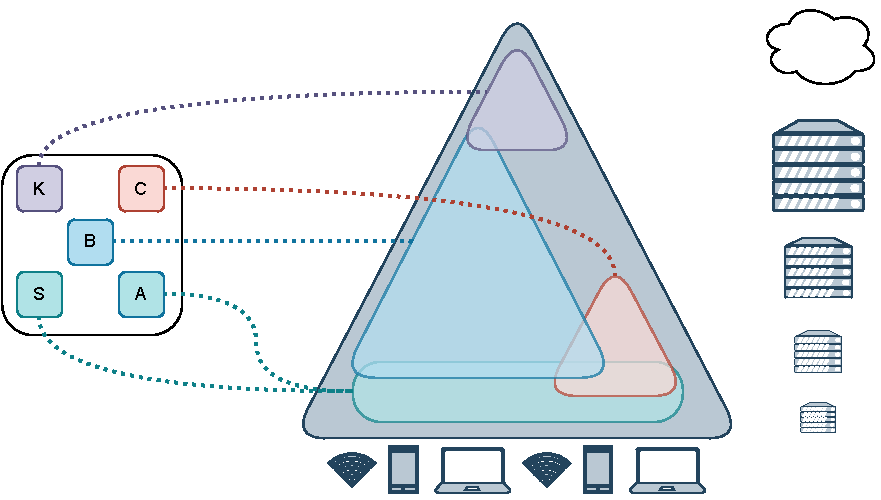
\includegraphics[width=.9\textwidth]{img/phd-proposal.drawio.pdf}
		\subcaption{Application decomposition via pulverization and dynamic reconfiguration in the edge-cloud continuum.}
	\end{minipage}
	\hfill
	\begin{minipage}[t]{0.45\textwidth}
		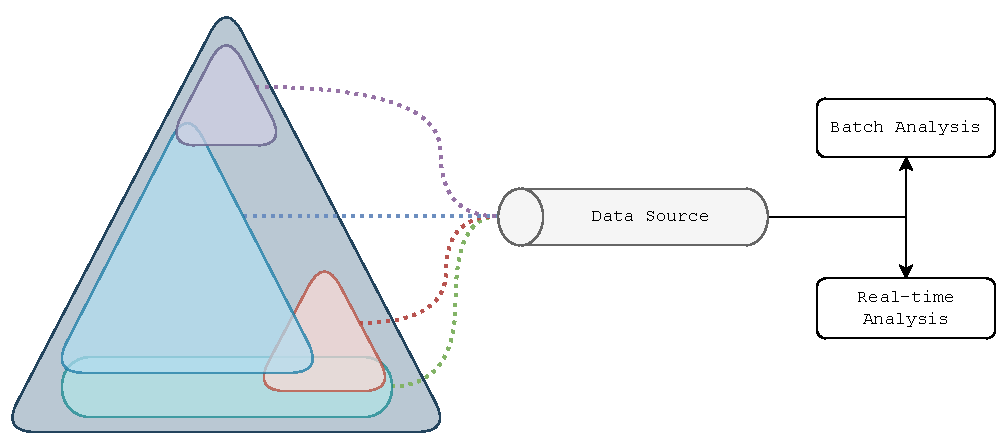
\includegraphics[width=.9\textwidth]{img/data-stream.drawio.pdf}
		\subcaption{Engineering of the data stream on heterogeneous infrastructure enabling different kinds of analysis.}
	\end{minipage}

	\caption{
		Overview of the project.
		Via pulverization the system is decomposed into components that can be independently deployed on the available infrastructure.
		The components can also be dynamically relocated into the infrastructure to adapt to changing conditions (left picture).
		Engineering of the data stream on heterogeneous infrastructure (right picture).
	}
	\label{fig:overview}
\end{figure}
%
One current limitation of this approach regards the runtime reconfiguration of the system based on the changing conditions or requirements.
%
This project aims to extend the current pulverisation approach to support dynamic reconfiguration of the system
by combining two approaches: \emph{Rule-based} and \emph{AI-based reconfiguration}.
%
The former can be used to define a set of static rules that can be used to reconfigure the system based on pre-determined and well-known conditions.
%
The latter can be extremely useful in contexts where the unpredictable conditions can be extremely high,
or where many different factors must be considered to determine the best configuration for the system.
%
The ability to dynamically reconfiguration is a fundamental aspect,
for example,
in contexts where energy-efficient systems are required,
or where the balance between consumption and performance can be strategic.

One other goal of this project is to bridge the gap between the simulation and the real world,
providing a set of \emph{methodology}, \emph{tools}, and \emph{techniques}
that can be seamlessly exploited to effectively tackle the system's complexity.

\ac{cas} can be composed of several different devices that can produce a large amount of data.
%
This kind of data can be characterized by many formats, different sources, and different frequencies.
%
The management of such data can be complicated and can lead to a large amount of data that cannot be processed with traditional techniques.
%
For this reason,
this project aims to provide a new approach to the engineering of data sources where a heterogeneous infrastructure is involved.
%
In this way,
the data can be available to be processed using big-data analysis techniques,
opening to new opportunities in the context of \ac{cas}.

As follows, is provided a brief overview of the main activities that will be carried out.

% -----------------
% Expected results
% -----------------

\section{Expected results}\label{sec:expected-results}

\paragraph{Pulverisation framework}
Realize an effective framework to support the development of complex systems
via the pulverisation approach.
%
We will provide a modular and extensible framework that can also be integrated with simulation tools
to allow the validation of the system before the deployment.

\paragraph{Rule-based system reconfiguration}
Extend the pulverisation approach and implement in the framework the possibility to
reconfigure the system at runtime.
%
The reconfiguration,
in the first phase,
will be carried out via a rule-based approach where the rules are defined by the user.

\paragraph{Dynamic system reconfiguration}
Integrate into the framework the possibility to adopt \ac{ai} techniques to automatically
manage the system reconfiguration at runtime.
%
The \ac{ai} can be strategically in contexts where complex \ac{qos} must be satisfied
performing better than a rule-based approach, that in some contexts can be too rigid.

\paragraph{Data stream engineering}
Enable the possibility to perform data analysis on the data produced by the system by providing
a data stream that ensemble the data produced by the devices in a heterogeneous system.
%
The data stream will be provided by the framework and can be used by the user to perform
data analysis leveraging,
for example,
big-data technologies.
%
The data stream engineering is bounded to the pulverisation approach,
in particular,
the data access is provided by the framework itself.

\paragraph{Integration with CAS frameworks}
Integrate the pulverisation framework with other, consolidated \ac{cas} frameworks
to provide a complete solution for the development and deployment of complex systems,
with the main focus on exploiting edge-cloud infrastructures.
%
\ac{ac} will be used as a possible solution for engineering \ac{cas},
and also as a possible case study for the framework validation.

% --------------------
% Activities
% --------------------

\section{Project activities}\label{sec:activities}

\subsection{First year goals}\label{subsec:first-year-activities}

The first-year goal,
based on the expected results reported in~\Cref{sec:expected-results},
are reported as follows.

\begin{itemize}
	\item Investigate the literature about many different approaches to the development of complex distributed systems,
	      for example, multi-tier programming and distributed reactive programming for engineering \ac{cas}.
	      Then, try to identify how these approaches can be integrated into the pulverization approach and possible improvements.
	\item Design and prototyping of a framework supporting the pulverization approach.
	      The framework will be designed to be modular and extensible but at the same time,
	      it should be easy to use and able to run on different platforms to support the development on heterogeneous systems.
	\item Integrate the framework with a reconfiguration engine to support the dynamic reconfiguration of the system.
	      The reconfiguration engine will be based on a rule-based approach allowing the user to specify the conditions in which the system should be reconfigured.
	      The reconfiguration rules can operate at different levels of granularity,
	      from the single device to the entire system.
\end{itemize}

\subsection{PhD goals}\label{subsec:phd-activities}

From~\Cref{sec:expected-results},
the remaining goals of the project are reported as follows.

\begin{itemize}
	\item Extend the reconfiguration model to support \ac{ai}-supported reconfiguration.
	      The \ac{ai} will be used to automatically reconfigure the system at runtime,
	      allowing the system to adapt to the changing conditions.
	      Several techniques can be adopted for this purpose,
	      for this reason,
	      we will investigate approaches ranging from RL to \ac{dl}.
	\item Integrate the pulverization framework with \ac{cas} frameworks to provide a full-stack solution for the design and deployment of this kind of system in heterogeneous infrastructures.
	      The main direction for this activity will be to investigate the integration with \ac{ac} frameworks,
	      for example,
	      ScaFi~\cite{DBLP:journals/softx/CasadeiVAP22} and Protelis~\cite{DBLP:conf/sac/PianiniVB15}.
	      These two frameworks are based on the aggregate programming paradigm,
	      which represents one possible way of engineering \ac{cas}.
	\item Due to the high volume of data produced by \ac{cas},
	      this project will try to investigate possible solutions to manage and engineer data sources,
	      to provide a way to effectively manage the data produced by the system.
	      %
	      This objective can be more challenging in a context where the infrastructure is heterogeneous,
	      and the data sources can be distributed across the infrastructure.
	      %
	      For this reason,
	      we will investigate a modern approach to serving data in a distributed and heterogeneous environment,
	      by integrating the pulverization framework with a data stream engine,
	      that can enable the possibility to perform data analysis on the data produced by the system.
\end{itemize}

\subsection{Scope}\label{subsec:scope}

\paragraph{Software engineering}
The challenges of the edge-cloud continuum lead to the need for new models,
design techniques, algorithms, languages, and tools to manage the complexity
of \ac{cps}.
%
With this new design approach,
there is the need to have the possibility to test and validate the system via simulation
and then seamlessly moves to the real deployments with a small effort.
%
This kind of seamless integration between simulation and real deployment can be strategic
to simplify the validation of the system and to reduce the time to market.

\paragraph{Distributed intelligence}
\ac{ai} is a computer science branch that has met big improvements over the last few years.
%
Even though the \ac{ai} usually tries to solve vertical and specific problems,
making it difficult to be applied in contexts like \ac{cas},
which are highly distributed by nature.
%
The value of a distributed intelligence leveraging \ac{ai} techniques can be strategic in \ac{cas},
in particular for adapting -- intelligently -- the system to changing conditions or to maintain certain \ac{qos}.

\paragraph{Energy and cost efficiency}
One of the current trends in the IT industry is the \emph{green computing}.
%
The need to reduce energy consumption and consequently the carbon footprint of the systems can be a requirement in many future systems.
%
For this reason,
supporting the design and implementation of systems in which from the many \ac{qos} parameters,
energy consumption is one of the most important,
must be a future direction of \ac{cps} and \ac{iot} systems.

\paragraph{Cyper-physical Systems}
We refer to \ac{cps} as a system that is composed of physical and computational components
that are deeply intertwined and interact with each other.
%
\emph{Smart cities}, \emph{Smart home}, \emph{Precision agricolture} are just some examples of \ac{cps}.
%
All of these systems can be very different from each other,
but they share some characteristics and challenges,
for example: \emph{dynamicity}, \emph{volume} (devices and produced data) and \emph{heterogeneity}.
%
The project can be framed in the context of \ac{cps} by providing an effective general solution to the aforementioned challenges,
which can be tailored to the specific needs of the system.

\subsection{Technology}\label{subsec:technology}

\paragraph{Cloud computing}
The objective of the pulverisation approach is to simplify the development and deployment of complex systems on diverse infrastructures.
%
The edge-cloud continuum,
a new paradigm,
combines the benefits of cloud and edge computing.
%
Understanding cloud computing and its technologies is crucial for designing and deploying such systems.
%
Popular cloud providers like Google \emph{Google Cloud Platform}~\footnote{\url{https://cloud.google.com/}},
\emph{Amazon Web Services}~\footnote{\url{https://aws.amazon.com/}},
and \emph{Microsoft Azure}~\footnote{\url{https://azure.microsoft.com/}} are the focus.
%
It's important to enable the framework to be compatible with multiple cloud providers.
%
Infrastructure provisioning has evolved to automation using tools like Terraform~\footnote{\url{https://www.terraform.io/}} and Ansible~\footnote{\url{https://www.ansible.com/}},
falling under the category of Infrastructure as Code (IaC).
%
These tools offer machine-readable infrastructure descriptions and APIs for programmatic interaction,
enabling integration with other tools and frameworks.
%
IaC facilitates dynamic, programmable, and automated deployment of the system on available infrastructure in the edge-cloud continuum.

% One of the main objectives of the pulverisation approach is to simplify the development
% and the deployment of complex systems on heterogeneous infrastructures.
% %
% The edge-cloud continuum is a new emerging paradigm that allows exploiting the
% advantages of both cloud and edge computing (and its continuum).
% %
% For this reason, it is fundamental to have a deep understanding of the cloud computing
% paradigm and its technologies to provide a complete solution for the design and deployment
% of this kind of system.
% %
% In recent years, several cloud providers have emerged, and each of them provides
% a set of services and technologies to support the development of cloud-based applications.
% %
% \emph{Google Cloud Platform}~\footnote{\url{https://cloud.google.com/}},
% \emph{Amazon Web Services}~\footnote{\url{https://aws.amazon.com/}},
% and \emph{Microsoft Azure}~\footnote{\url{https://azure.microsoft.com/}}
% are the most popular cloud providers, and they will be the main focus of this project.
% %
% Could be strategic to enable the framework to be used with different cloud providers
% to allow the user to choose the one that best suits his needs.
% %
% In recent years,
% the way to provision infrastructure has changed.
% %
% The trend is to fully automate the provisioning of the infrastructure via dedicated tools,
% like Terraform~\footnote{\url{https://www.terraform.io/}} and Ansible~\footnote{\url{https://www.ansible.com/}}.
% %
% These tools fall in the category of \ac{iac}: they allow to describe the infrastructure in a machine-readable format
% instead of using interactive configuration tools.
% %
% Moreover,
% these tools provide a set of \ac{api} to interact with them programmatically,
% allowing the integration with other tools and frameworks.
% %
% As a consequence,
% these tools can be used in a \ac{ci} pipeline to fully automate the deployment of the system.
% %
% \ac{iac} represents a powerful technology in the context of the edge-cloud continuum,
% allowing a dynamic, programmable and automated deployment of the system on the available infrastructure.

\paragraph{Data stream}
The \ac{iot} systems consist of a large number of devices that produce a large amount of data
from extremely scattered data sources.
%
The handling of such data requires an adequate infrastructure and tools to manage them.
%
For this reason, the project will investigate the use of big-data technologies
such as \emph{Apache Spark}~\footnote{\url{https://spark.apache.org/}},
\emph{Apache Flink}~\footnote{\url{https://flink.apache.org/}} and their integration with the pulverisation approach and the \ac{ac} frameworks.
%
The union of big-data technologies and the pulverisation approach can open new opportunities for \ac{cas}.

\paragraph{Distributed technology}
The resilience of the system is a fundamental aspect to consider when designing
and deploying a collective adaptive application.
%
Due to the highly distributed nature of the \ac{iot} and \ac{ac} systems,
the failure of a node is the norm rather than the exception.
%
For this reason, will be investigated the use of distributed technologies like \emph{MOM},
specifically, RabbitMQ~\footnote{\url{https://www.rabbitmq.com/}} and ZeroMQ~\footnote{\url{https://zeromq.org/}};
microservices patterns and approaches to provide a resilient system.
%
Orchestration tools like Kubernetes~\footnote{\url{https://kubernetes.io/}} can be used to manage the deployment of the system
and the dynamic reconfiguration of it.

\subsection{Long-term contribution}
The initiative proposed in this project aims to tackle the complexity of designing and deploying systems on heterogeneous infrastructures,
where the main focus is on \ac{cas}.
%
Beyond the specific contribution of the project,
which the main focus is on the pulverisation approach,
I expect to contribute to the research community providing new approaches and solutions to the aforementioned challenges.
%
In particular,
I expect to provide a deep understanding of the role of \ac{cas} in modern scenarios like \emph{smart cities}, \emph{large scale \ac{iot} systems}, and so on,
and providing reference implementations of the proposed approaches.
%
Summing up,
this project can be seen as a groundwork for the creation of systems in the edge-cloud continuum where dynamicity and self-adaptation are key aspects.
%
\ac{ai} and data analysis cover a fundamental role in this context,
enabling a new set of opportunities that this project aims to explore.

\newpage

\printbibliography

\end{document}
